% IEEE standard conference template; to be used with:
%   spconf.sty  - LaTeX style file, and
%   IEEEbib.bst - IEEE bibliography style file.
% --------------------------------------------------------------------------

\documentclass[letterpaper]{article}
\usepackage{spconf,amsmath,amssymb,graphicx}

% Example definitions.
% --------------------
% nice symbols for real and complex numbers
\newcommand{\R}[0]{\mathbb{R}}
\newcommand{\C}[0]{\mathbb{C}}

% bold paragraph titles
\newcommand{\mypar}[1]{{\bf #1.}}

% Title.
% ------
\title{A Descriptive Title, not too general, not too long}
%
% Single address.
% ---------------
\name{Markus P\"uschel\thanks{The author thanks Jelena Kovacevic. This paper
is a modified version of the template she used in her class.}} 
\address{Department of Computer Science\\ ETH Z\"urich\\Z\"urich, Switzerland}

% For example:
% ------------
%\address{School\\
%		 Department\\
%		 Address}
%
% Two addresses (uncomment and modify for two-address case).
% ----------------------------------------------------------
%\twoauthors
%  {A. Author-one, B. Author-two\sthanks{Thanks to XYZ agency for funding.}}
%		 {School A-B\\
%		 Department A-B\\
%		 Address A-B}
%  {C. Author-three, D. Author-four\sthanks{The fourth author performed the work
%		 while at ...}}
%		 {School C-D\\
%		 Department C-D\\
%		 Address C-D}
%

\begin{document}
%\ninept
%
\maketitle
%

The hard page limit is 6 pages in this style. Do not reduce font size
or use other tricks to squeeze. This pdf is formatted in the American letter format, so the spacing may look a bit strange when printed out.

\begin{abstract}
Describe in concise words what you do, why you do it (not necessarily
in this order), and the main result.  The abstract has to be
self-contained and readable for a person in the general area. You
should write the abstract last.
\end{abstract}

\section{Introduction}\label{sec:intro}

Do not start the introduction with the abstract or a slightly modified
version. It follows a possible structure of the introduction. 
Note that the structure can be modified, but the
content should be the same. Introduction and abstract should fill at most the first page, better less.

\mypar{Motivation} The first task is to motivate what you do.  You can
start general and zoom in one the specific problem you consider.  In
the process you should have explained to the reader: what you are doing,
why you are doing, why it is important (order is usually reversed).

For example, if my result is the fastest sorting implementation ever, one
could roughly go as follows. First explain why sorting is important
(used everywhere with a few examples) and why performance matters (large datasets,
realtime). Then explain that fast implementations are very hard and
expensive to get (memory hierarchy, vector, parallel). 

Now you state what you do in this paper. In our example: 
presenting a sorting implementation that is
faster for some sizes as all the other ones.

\mypar{Related work} Next, you have to give a brief overview of
related work. For a report like this, anywhere between 2 and 8
references. Briefly explain what they do. In the end contrast to what
you do to make now precisely clear what your contribution is.

\section{Background: Whatever the Background is}\label{sec:background}

Give a short, self-contained summary of necessary
background information. For example, assume you present an
implementation of sorting algorithms. You could organize into sorting
definition, algorithms considered, and asymptotic runtime statements. The goal of the
background section is to make the paper self-contained for an audience
as large as possible. As in every section
you start with a very brief overview of the section. Here it could be as follows: In this section 
we formally define the sorting problem we consider and introduce the algorithms we use
including a cost analysis.

\mypar{Sorting}
Precisely define sorting problem you consider.

\mypar{Sorting algorithms}
Explain the algorithm you use including their costs.

As an aside, don't talk about "the complexity of the algorithm.'' It's incorrect,
problems have a complexity, not algorithms.


\section{Your Proposed Method}\label{sec:yourmethod}

Now comes the ``beef'' of the report, where you explain what you
did. Again, organize it in paragraphs with titles. As in every section
you start with a very brief overview of the section.

In this section, structure is very important so one can follow the technical content.

Mention and cite any external resources that you used including libraries or other code.

\section{Experimental Results}\label{sec:exp}

In order to evaluate the efficiency of our proposed algorithms, we tested them on sets of randomly generated points with different geometric shapes: square, disk and circle.

Regarding scalability we tested both weak and strong scaling, changing the input size and the number of operating threads.

Concerning correctness we compared our results with the ones obtained using th \textit{Convex Hull} implementation available in the library \textit{CGAL}.

\mypar{Experimental setup}

Xeon Phi (momentarily my pc lol)
%TODO
 Specify the platform (processor, frequency, maybe OS, maybe cache sizes)
as well as the compiler, version, and flags used. If your work is about performance, 
I strongly recommend that you play with optimization flags and consider also icc for additional potential speedup.
\begin{table}[!ht]
\begin{tabular}{|c|c|}
\hline Architecture: 		 & x86$\_$64\\
\hline CPU op-mode(s):        & 32-bit, 64-bit\\
\hline CPU(s):                & 8\\
\hline Thread(s) per core:    & 2\\
\hline Core(s) per socket:    & 4\\
\hline Socket(s):             & 1\\
\hline Model name:            & Intel(R) Core(TM) i7-6700HQ\\							 & CPU @ 2.60GHz\\
\hline CPU MHz:               & 800.007\\
\hline CPU max MHz:           & 3500.0000\\
\hline CPU min MHz:           & 800.0000\\
\hline L1d cache:             & 32K\\
\hline L1i cache:             & 32K\\
\hline L2 cache:              & 256K\\
\hline L3 cache:              & 6144K\\
\hline
\end{tabular}
\caption{Xeon Phi cluster specifications}
\end{table}

Our implementations are written in \textit{C++} and make use of \textit{OpenMP} for shared-memory multithreading.
Our applications were compiled using \textit{icc} with the flag \textit{-O2}.

This is roughly how our experiments worked:
First of all we fixed a shape and a number of points to be generated. Then we randomly generated the chosen point set and executed each algorithm with each desired number of threads on that point set, collecting results in logfiles, measuring two time intervals: mid and end.

In order to have reliable experiments we repeated this process 100 times for each chosen combination of number of input points and shape.

This whole process was done for 10K, 100K, 1M and 10M points generated in a range R of 1B and as shapes we used a square, a disk and a circumference in the following way:
\mypar{Square}: Randomly generated points with coordinates in the range [-R,R]
\mypar{Disk}: Randomly generated points with coordinates in the range [-R,R]. Points not included in the disk with radius R and center (0,0) were removed and regenerated.
\mypar{Circle}: Randomly generated angles $\theta_n$ and created the points ($\frac{R}{2}cos(\theta_n)$, $\frac{R}{2}sin(\theta_n)$).

\mypar{Results}

Next divide the experiments into classes, one paragraph for each. In each class of experiments you typically pursue one questions that then is answered by a suitable plot or plots. For example, first you may want to investigate the performance behavior with changing input size, then how your code compares to external benchmarks.

\mypar{General results and reliability}

Put BOXPLOTS HERE

\mypar{Change input size}

For the sequential versions, as expected, the growth in execution time when increasing the number of input points is linear for all the selected shapes.
For the parallel algorithms, instead, the situation slightly differs.

For square and disk they all behave similarly: the effeciency grows when incrementing the input size for less than 1M input points. With a higher number of points ($\geq$ 1M) the execution time grows linearly and it's very similar for all the considered algorithms.

\begin{figure}[!ht]\centering
  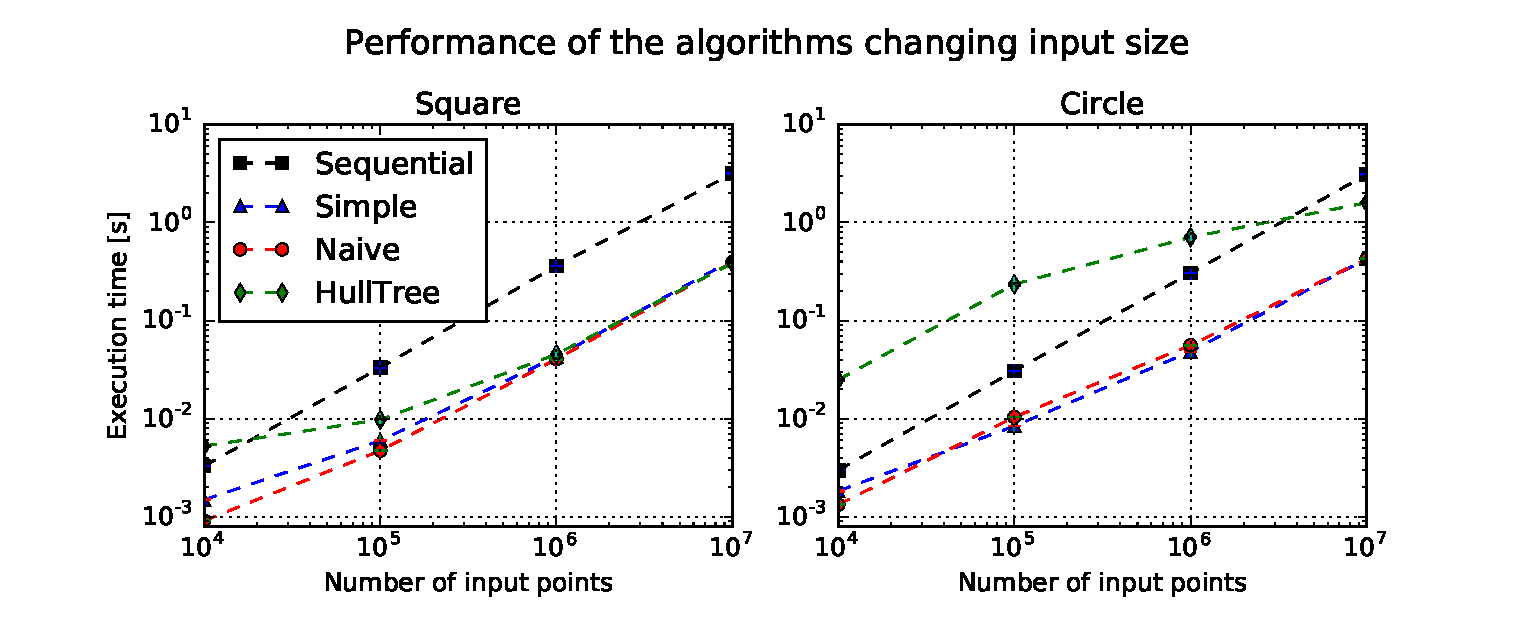
\includegraphics[scale=0.33]{./plots/time_points.eps}
  \caption{Comparison of the execution times three algorithms for 8 threads and the sequential version changing input size for square and circle\label{Input size time}}
\end{figure}

Regarding circle, instead, \textit{Pairwise} and \textit{Naive} algorithms have a performance comparable to the one on the square, while \textit{HullTree}'s performance is much worse.
This is due to the creation of the data structure that for a high number of resulting points (recall that for circle every generated point is part of the final convex hull) needs a lot of time.

\begin{figure}[!ht]\centering
  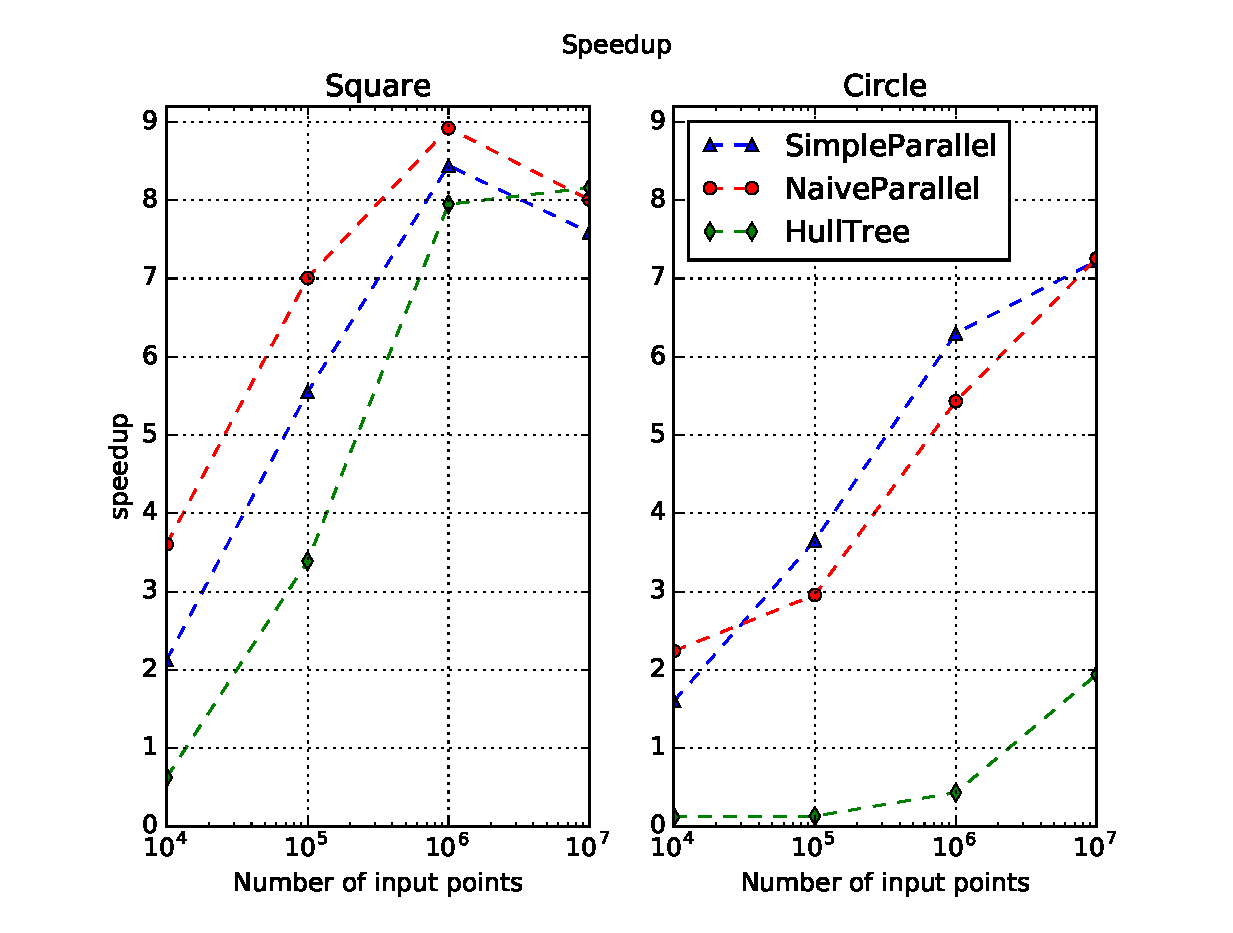
\includegraphics[scale=0.33]{./plots/speedup_points.eps}
  \caption{Speedup comparison of the three algorithms for 8 threads changing input size for square and circle\label{Input size speedup}}
\end{figure}

It must be noticed that the parallel algorithms have a better speedup when the number of points increases, meaning that the bigger the input set, the better the performance optimization introduced by the parallelization.

\mypar{Change Threads num}

Considering an input set of 1M and 10M points, for square and disk we obtained very good results when changing the number of working threads: for 2 and 4 threads we even obtained superlinear speedup with the HullTree algorithm.
A good speedup is still visible over 8 threads but we lose efficiency over a certain limit, past that the overhead added by parallelism cannot overweights the benefits introduced by reducing the problem's size.

We can notice that that point is shifted to a higher number of threads when the input set is bigger. Clearly the lower the number of points the lesser the efficiency obtained by splitting the point set among threads.

\begin{figure}[!ht]\centering
  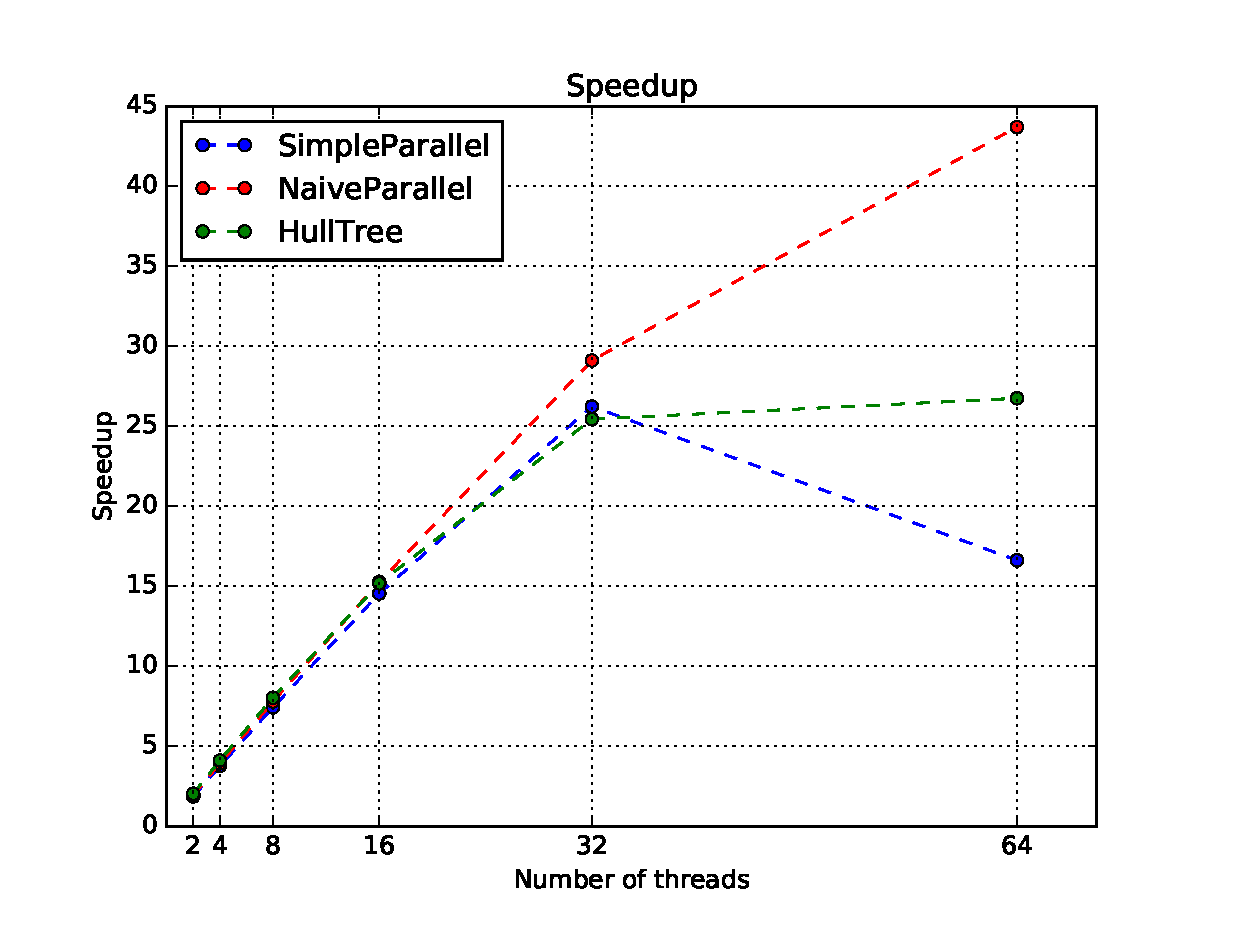
\includegraphics[scale=0.33]{./plots/speedup_xeon_square_10000000.eps}
  \caption{Speedup of the algorithms with the given number of threads with a square for 1M and 10M points\label{Threads time}}
\end{figure}

For circle the situation is again more complicated, since the HullTree algorithm has a very bad performance.
The other algorithms still have decent speedups but not as good as with the square.
The more memory accesses needed and the parallel overhead are make the algorithms scale worse.



We can notice that for X threads the algorithms stop scaling.

\mypar{Behavior with unoptimal number of threads}

Here we show the behavior of HullTree and Simple algirthms with a number of threads which is sot a power of two. Unfortunately, Naive algorithm cannot work with these numbers of threads.

\begin{figure}[!ht]\centering
  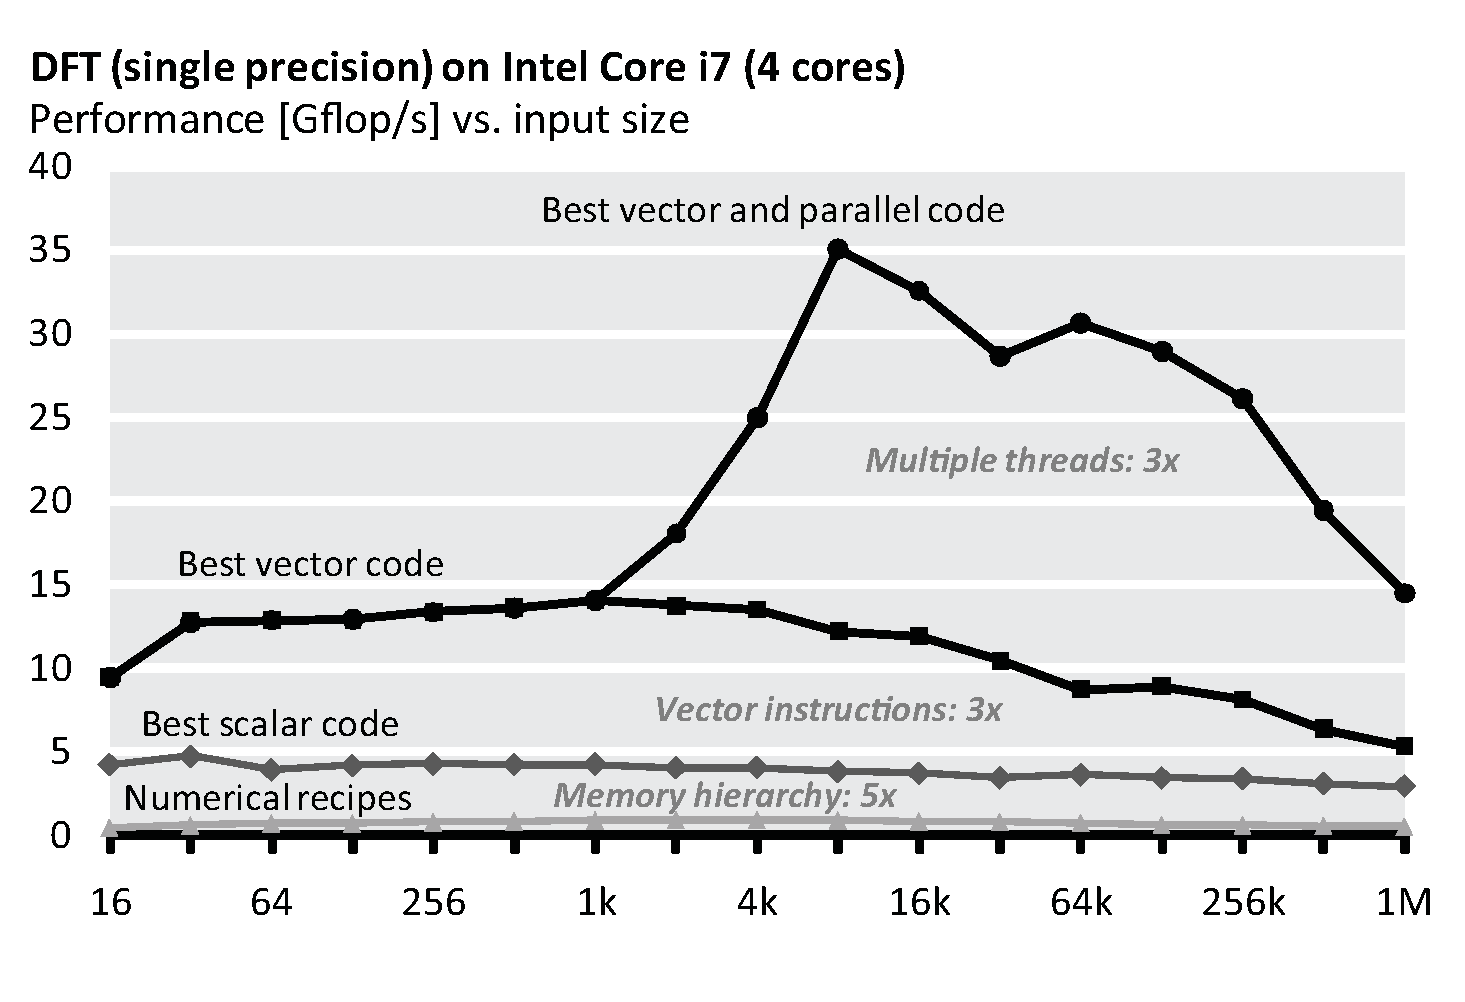
\includegraphics[scale=0.33]{dft-performance.eps}
  \caption{Execution times of the algorithms with the given number of threads for an input set of 10M points in a square on Xeon Phi and Euler\label{fftperf}}
\end{figure}

The algorithms behave in some way lol, that way is a way for Simple, whereas for HullTree we have a different way.

For some tips on benchmarking including how to create a decent viewgraph see pages 22--27 in \cite{Pueschel:10}.

{\bf Comments:}
\begin{itemize}
\item Create very readable, attractive plots (do 1 column, not 2 column plots
for this report) with readable font size. However, the font size should also not be too large; typically it is smaller than the text font size.
An example is in Fig.~\ref{fftperf} (of course you can have a different style).
\item Every plot answers a question. You state this question and extract the
answer from the plot in its discussion.
\item Every plot should be referenced and discussed.
\end{itemize}

\section{Conclusions}

Here you need to summarize what you did and why this is
important. {\em Do not take the abstract} and put it in the past
tense. Remember, now the reader has (hopefully) read the report, so it
is a very different situation from the abstract. Try to highlight
important results and say the things you really want to get across
such as high-level statements (e.g., we believe that .... is the right
approach to .... Even though we only considered x, the
.... technique should be applicable ....) You can also formulate next
steps if you want. Be brief. After the conclusions there are only the references.

\section{Further comments}

Here we provide some further tips.

\mypar{Further general guidelines}

\begin{itemize}
\item For short papers, to save space, I use paragraph titles instead of
subsections, as shown in the introduction.

\item It is generally a good idea to break sections into such smaller
units for readability and since it helps you to (visually) structure the story.

\item The above section titles should be adapted to more precisely
reflect what you do.

\item Each section should be started with a very
short summary of what the reader can expect in this section. Nothing
more awkward as when the story starts and one does not know what the
direction is or the goal.

\item Make sure you define every acronym you use, no matter how
convinced you are the reader knows it.

\item Always spell-check before you submit (to us in this case).

\item Be picky. When writing a paper you should always strive for very
high quality. Many people may read it and the quality makes a big difference.
In this class, the quality is part of the grade.

\item Books helping you to write better: \cite{Higham:98} and \cite{Strunk:00}.

\item Conversion to pdf (latex users only): 

dvips -o conference.ps -t letter -Ppdf -G0 conference.dvi

and then

ps2pdf conference.ps
\end{itemize}

\mypar{Graphics} For plots that are not images {\em never} generate the bitmap formats
jpeg, gif, bmp, tif. Use eps, which means encapsulate postscript. It is
scalable since it is a vector graphic description of your graph. E.g.,
from Matlab, you can export to eps.

The format pdf is also fine for plots (you need pdflatex then), but only if the plot was never before in the format 
jpeg, gif, bmp, tif.


% References should be produced using the bibtex program from suitable
% BiBTeX files (here: bibl_conf). The IEEEbib.bst bibliography
% style file from IEEE produces unsorted bibliography list.
% -------------------------------------------------------------------------
\bibliographystyle{IEEEbib}
\bibliography{bibl_conf}

\end{document}

